\documentclass[xelatex,ja=standard]{bxjsarticle}
\setCJKmainfont[BoldFont=NotoSerifCJKjp-Black]{NotoSerifCJKjp-Light}
\setCJKsansfont[BoldFont=NotoSansCJKjp-Black]{NotoSansCJKjp-Light}
\setCJKmonofont[BoldFont=NotoSansCJKjp-Black]{NotoSansCJKjp-Light}
\usepackage{physics}
\usepackage{bm}
\usepackage[colorlinks=true, linkcolor=black, citecolor=black, urlcolor=blue]{hyperref}
\usepackage{graphicx}



\title{シュレーディンガー方程式を有限要素法で解く}
\author{山本峻介}
\date{\today}

\begin{document}

\maketitle

\section{水素原子}
\subsection{シュレーディンガー方程式}
水素原子のシュレーディンガー方程式は
\begin{align}
    \qty(-\frac{\hbar^2}{2\mu}\nabla^2 -\frac{e^2}{4\pi\epsilon_0 r})\psi = E\psi
\end{align}
である。無次元量$R, E_0$により、
\begin{align}
    r = R\tilde{r},\quad E = E_0\varepsilon
\end{align}
と変換すると、
\begin{align}
    \qty(-\frac{1}{2}\tilde\nabla^2 - \frac{\mu R e^2}{\hbar^2 4\pi\epsilon_0}\frac{1}{\tilde r})\psi = \frac{\mu E_0R^2}{\hbar^2}\varepsilon\psi
\end{align}
となる。ここで、
\begin{align}
    R = \frac{\hbar^2 4\pi\epsilon_0}{\mu e^2}, \quad E_0 = \frac{\hbar^2}{\mu R^2}
\end{align}
とすれば、
\begin{align}
    \qty(-\frac{1}{2}\tilde\nabla^2 - \frac{1}{\tilde r})\psi = \varepsilon\psi\label{eq:dimless}
\end{align}
となる。$R$はボーア半径である。

(\ref{eq:dimless})の動経成分は
\begin{align}
    \qty[-\frac{1}{2}\qty(\frac{1}{r^2}\dv{r}r^2\dv{r} - \frac{l(l+1)}{r^2})
     - \frac{1}{r}]R = \varepsilon R
\end{align}
となる。$\chi = rR$を導入すると、
\begin{align}
    -\frac{1}{2}\qty(\dv[2]{r} - \frac{l(l+1)}{r^2})\chi - \frac{1}{r}\chi = \varepsilon\chi
\end{align}
となる。 

\subsection{弱形式}
次の固有方程式
\begin{align}
    \qty(\dv[2]{x} + v(x))f = \lambda f\label{eq:eigen}
\end{align}
の弱解を求める。$f$に対してテスト関数$g$を掛けて積分すると、
\begin{align}
    \int_0^Lg\qty(\dv[2]{x} + v)f\dd{x} &= \lambda\int_0^Lgf\dd{x}\notag\\
    \qty[g\dv{f}{x}]_0^L+\int_0^L\qty(-\dv{g}{x}\dv{f}{x} + gvf)\dd{x}
     &= \lambda\int_0^Lgf\dd{x}\label{eq:weak}
\end{align}
となる。  任意の$g$に対して(\ref{eq:weak})が成り立つとき、$f$は(\ref{eq:eigen})の弱解である。
\subsection{有限要素法}
\subsubsection{$v$に特異性がない場合}
%(\ref{eq:weak})の被積分関数は、$\dv{g}{x}\dv{f}{x}$と$h(x)g(x)f(x)$からなる。
補完関数
\begin{align}
    N_p(x) = 
    \begin{cases}
        \dfrac{x-x_{p-1}}{h_{p-1}}&x_{p-1}<x<x_p,\\
        \dfrac{x_{p+1} - x}{h_p}&x_{p}<x<x_{p+1},\\
        0&\text{otherwise},
    \end{cases}
\end{align}
を導入する。$g(x) = \sum_{p=1}^N g_pN_p(x)$, $f(x) = \sum_{q=1}^N f_qN_q(x)$と近似すると、
\begin{align}
    -\int_0^L \dv{g}{x}\dv{f}{x}\dd{x}
     =& -\sum_{p, q}g_pf_q\bigg(\delta_{p - 1, q}\dfrac{-1}{h_{p-1}}\cdot\dfrac{1}{h_{p-1}}\cdot h_{p-1}
      + \delta_{q, p}\qty(\dfrac{1}{h_{p-1}}\cdot\dfrac{1}{h_{p-1}}\cdot h_{p-1} + \dfrac{-1}{h_{p}}\cdot\dfrac{-1}{h_{p}}\cdot h_{p})\notag\\
      &+ \delta_{q, p + 1}\dfrac{1}{h_{p}}\cdot\dfrac{-1}{h_{p}}\cdot h_{p}
      \bigg)\notag\\
     =& \sum_{p, q}g_pf_q\bigg(\delta_{q, p - 1}\dfrac{1}{h_{p-1}}
      + \delta_{q, p}\qty(\dfrac{-1}{h_{p-1}} + \dfrac{-1}{h_{p}})+ \delta_{q, p + 1}\dfrac{1}{h_{p}}
      \bigg),
\end{align}
\begin{align}
    \int_0^L gf\dd{x}
     =& \sum_{p, q}g_pf_q\bigg(\delta_{q, p - 1}\int_{x_{p-1}}^{x_p}\dfrac{x_{p} - x}{h_{p-1}}\cdot\dfrac{x-x_{p-1}}{h_{p-1}}\dd{x}\notag\\
      &+ \delta_{q, p}\qty(\int_{x_{p-1}}^{x_p}\dfrac{x-x_{p-1}}{h_{p-1}}\cdot\dfrac{x-x_{p-1}}{h_{p-1}}\dd{x}
       + \int_{x_{p}}^{x_{p+1}}\dfrac{x_{p+1} - x}{h_{p}}\cdot\dfrac{x_{p+1} - x}{h_{p}}\dd{x})\notag\\
      &+ \delta_{q, p + 1}\int_{x_{p}}^{x_{p+1}}\dfrac{x-x_{p}}{h_{p}}\cdot\dfrac{x_{p+1} -x}{h_{p}}\cdot h_{p}
      \bigg)\notag\\
      =& \sum_{p, q}g_pf_q\bigg(\delta_{q, p - 1}\dfrac{h_{p-1}}{6}
      + \delta_{q, p}\qty(\dfrac{h_{p-1}}{3} + \dfrac{h_{p}}{3})+ \delta_{q, p + 1}\dfrac{h_{p}}{6}\bigg),
\end{align}
\begin{align}
    \int_0^L& vgf\dd{x}\notag\\
     =& \sum_{p, q}g_pf_q\bigg(\delta_{q, p - 1}v_{p-1}\int_{x_{p-1}}^{x_p}\dfrac{\qty(x-x_{p-1})\qty(x_{p} - x)^2}{h_{p-1}^3}\dd{x}\notag\\
    &+\delta_{q, p - 1}v_{p}\int_{x_{p-1}}^{x_p}\dfrac{\qty(x-x_{p-1})^2\qty(x_{p} - x)}{h_{p-1}^3}\dd{x}\notag\\
    &+\delta_{q, p}v_{p-1}\int_{x_{p-1}}^{x_p}\dfrac{\qty(x-x_{p-1})^2\qty(x_{p} - x)}{h_{p-1}^3}\dd{x}\notag\\
    &+\delta_{q, p}v_{p}\int_{x_{p-1}}^{x_p}\dfrac{\qty(x-x_{p-1})^3}{h_{p-1}^3}\dd{x}\notag\\
    &+\delta_{q, p}v_{p}\int_{x_{p}}^{x_{p+1}}\dfrac{\qty(x_{p+1} - x)^3}{h_{p}^3}\dd{x}\notag\\
    &+\delta_{q, p}v_{p+1}\int_{x_{p}}^{x_{p+1}}\dfrac{\qty(x_{p+1} - x)^2\qty(x-x_{p})}{h_{p}^3}\dd{x}\notag\\
    &+\delta_{q, p+1}v_{p}\int_{x_{p}}^{x_{p+1}}\dfrac{\qty(x_{p+1} - x)^2\qty(x-x_{p})}{h_{p}^3}\dd{x}\notag\\
    &+\delta_{q, p+1}v_{p+1}\int_{x_{p}}^{x_{p+1}}\dfrac{\qty(x_{p+1} - x)\qty(x-x_{p})^2}{h_{p}^3}\dd{x}\notag\\
    \bigg)\notag\\
    =& \sum_{p, q}g_pf_q\bigg(\delta_{q, p - 1}v_{p-1}\frac{h_{p-1}}{12}+\delta_{q, p - 1}v_{p}\frac{h_{p-1}}{12}+\delta_{q, p}v_{p-1}\frac{h_{p-1}}{12} +\delta_{q, p}v_{p}\frac{h_{p-1}}{4}\notag\\
    &+\delta_{q, p}v_{p}\frac{h_{p}}{4} + \delta_{q, p}v_{p+1}\frac{h_p}{12}+\delta_{q, p+1}v_{p}\frac{h_p}{12}+\delta_{q, p+1}v_{p+1}\frac{h_{p}}{12}\bigg)\notag\\
    =& \frac{1}{12}\sum_{p, q}g_pf_q\bigg(\delta_{q, p - 1}h_{p-1}\qty(v_{p-1} + v_p)+\delta_{q, p}h_{p-1}\qty(v_{p-1} + 3v_p) \notag\\
    &+\delta_{q, p}h_{p}\qty(3v_p + v_{p+1})+\delta_{q, p+1}h_p\qty(v_{p} + v_{p+1})\bigg)\notag\\
\end{align}
\begin{align}
    \int_0^L vgf\dd{x}
    =& \sum_{l=1}^N \frac{1}{{h^l}^3}\int_{x^l_0}^{x^l_1}
    \qty(\qty(x^l_1 - x)v^l_0 + \qty(x-x^l_0)v^l_1)
    \qty(\qty(x^l_1 - x)g^l_0 + \qty(x-x^l_0)g^l_1)\notag\\
    &\times\qty(\qty(x^l_1 - x)f^l_0 + \qty(x-x^l_0)f^l_1)
    \dd{x}\notag\\
    =& \sum_{l=1}^N \frac{1}{{h^l}^3}\int_{x^l_0}^{x^l_1}
    \mqty(g^l_0 & g^l_1) \mqty(x^l_1 - x \\ x-x^l_0)
    \qty(\qty(x^l_1 - x)v^l_0 + \qty(x-x^l_0)v^l_1)\notag\\
    &\times\mqty(x^l_1 - x & x-x^l_0)\mqty(f^l_0 \\ f^l_1)
    \dd{x}\notag\\
    =& \frac{1}{12}\sum_{l=1}^N h^l
    \mqty(g^l_0 & g^l_1) \mqty(3v_0^l +v_1^l & v_0^l +v_1^l\\ v_0^l +v_1^l&v_0^l +3v_1^l)\mqty(f^l_0 \\ f^l_1),
\end{align}
となる。(\ref{eq:weak})は
\begin{align}
    \sum_{l=1}^N \mqty(g^e_0 & g^e_1)\bigg[\frac{1}{h^l}\mqty(1 & -1 \\ -1 & 1)
     + \frac{h^l}{12}\mqty(3v_{0}^l +v_{1}^l & v_{0}^l +v_{1}^l\\ v_{0}^l +v_{1}^l&v_{0} +3v_{1}^l)\bigg]\mqty(f^l_0 \\ f^l_1)=\lambda\sum_{l=1}^N \frac{h^l}{6} \mqty(g^l_0 & g^l_1)\mqty(2 & 1\\1& 2)\mqty(f^l_0 \\ f^l_1)
\end{align}
となる。 任意の$g$に対して上式が成り立つとき、
\begin{align}
    \sum_{l=1}^N \bigg[\frac{1}{h^l}\mqty(1 & -1 \\ -1 & 1)
     + \frac{h^l}{12}\mqty(3v_{0}^l +v_{1}^l & v_{0}^l +v_{1}^l\\ v_{0}^l +v_{1}^l&v_{0}^l +3v_{1}^l)\bigg]\mqty(f^l_0 \\ f^l_1)&=\lambda\sum_{l=1}^N\frac{h^l}{6} \mqty(2 & 1\\1& 2)\mqty(f^l_0 \\ f^l_1)
\end{align}     
左辺第1項の行列を$K$, 第2項の行列を$V$、右辺の行列を$M$、 固有関数の列を$u$とすると、
\begin{align}
    K&=
     \mqty(
     \frac{1}{h_0} & -\frac{1}{h_0} & 0 & \cdots & 0 & 0 & 0 \\
     -\frac{1}{h_0} & \frac{1}{h_0} + \frac{1}{h_1} & -\frac{1}{h_1} & \cdots & 0 & 0 & 0 \\
     0 & -\frac{1}{h_1} & \frac{1}{h_1} + \frac{1}{h_2} & \cdots & 0 & 0 & 0 \\
     \vdots & \vdots & \vdots & \ddots & \vdots  & \vdots& \vdots\\
     0 & 0 & 0 & \cdots & \frac{1}{h_{N-2}} + \frac{1}{h_{N-1}} & -\frac{1}{h_{N-1}} & 0 \\
     0 & 0 & 0 & \cdots & -\frac{1}{h_{N-1}} &\frac{1}{h_{N-1}} + \frac{1}{h_N} & -\frac{1}{h_N} \\
     0 & 0 & 0 & \cdots & 0 & -\frac{1}{h_N}& \frac{1}{h_N} \\
     ),
\end{align}
\begin{align}
     V&= \frac{1}{12}\left(\mqty{
        \qty(3v_{0} +v_{1})h_0 & \qty(v_{0} +v_{1})h_0 & 0 & \cdots \\
        \qty(v_{0} +v_{1})h_0 & \qty(v_{0} + 3v_{1})h_0 + \qty(3v_{1} +v_{2})h_1 & \qty(v_{1} +v_{2})h_1 & \cdots\\
        0 & \qty(v_{1} +v_{2})h_1 & \qty(v_{1} + 3v_{2})h_1 + \qty(3v_{2} + v_{3})h_2 & \cdots\\
        \vdots & \vdots & \vdots & \ddots\\
        0 & 0 & 0 & \cdots\\
        0 & 0 & 0 & \cdots\\
        }\right.\notag\\
     &  \left.\mqty{
        \cdots  & 0 & 0 & 0 \\
        \cdots & 0 & 0 & 0 \\
        \cdots& 0 & 0 & 0 \\
        \ddots  & \vdots& \vdots& \vdots\\
        \cdots & h_{N-2}\qty(v_{N-2} + 3v_{N-1}) + h_{N-1}\qty(3v_{N-1} + v_{N})& h_{N-1}\qty(v_{N - 1} +v_{N})& 0 \\
        \cdots & h_{N-1}\qty(v_{N - 1} +v_{N})& h_{N-1}\qty(v_{N-1} + 3v_{N}) + h_N\qty(3v_{N} + v_{N +1})& h_N\qty(v_{N} +v_{N+1}) \\
        \cdots &0 & h_N\qty(v_{N} +v_{N+1})& h_N\qty(v_{N} +3v_{N+1}) \\
        }\right),
\end{align}
\begin{align}
    M&=
     \frac{1}{6}\mqty(
     2h_0 & h_0 & 0 & \cdots & 0 & 0 & 0 \\
     h_0 & 2h_0 + 2h_1 & h_1 & \cdots & 0 & 0 & 0 \\
     0 & h_1 & 2h_1 + 2h_2 & \cdots & 0 & 0 & 0 \\
     \vdots & \vdots & \vdots & \ddots & \vdots  & \vdots& \vdots\\
     0 & 0 & 0 & \cdots & 2h_{N - 2} + 2h_{N - 1} & h_{N-1}& 0 \\
     0 & 0 & 0 & \cdots & h_{N-1} & 2h_{N - 1} + 2h_{N}& h_{N} \\
     0 & 0 & 0 & \cdots & 0 & h_{N}& 2h_{N} \\
     ),
\end{align}
\begin{align}
    u&=\mqty(f_0 & f_1 & \cdots & f_N & f_{N+1})^T
\end{align}
となる。ただし、$f_N^0 = f_N,\, f_N^1 = f_{N+1}$($v$についても同様)である。これらから、
\begin{align}
    \qty(K + V) u = \lambda Mu 
\end{align}
となる。

ディリクレ境界条件$f(0) = f_0 = 0$, $f(L) = f_{N+1} = 0$を課すと
\begin{align}
    K&=
     \mqty(
     \frac{1}{h_0} + \frac{1}{h_1} & -\frac{1}{h_1} & \cdots & 0 & 0\\
     -\frac{1}{h_1} & \frac{1}{h_1} + \frac{1}{h_2} & \cdots & 0 & 0\\
     \vdots & \vdots & \vdots & \ddots & \vdots\\
     0 & 0 & \cdots & \frac{1}{h_{N-2}} + \frac{1}{h_{N-1}} & -\frac{1}{h_{N-1}} \\
     0 & 0 & \cdots & -\frac{1}{h_{N-1}} &\frac{1}{h_{N-1}} + \frac{1}{h_N} \\
     ),
\end{align}
\begin{align}
     V&= \frac{1}{12}\left(\mqty{
        \qty(v_{0} + 3v_{1})h_0 + \qty(3v_{1} +v_{2})h_1 & \qty(v_{1} +v_{2})h_1 & \cdots\\
        \qty(v_{1} +v_{2})h_1 & \qty(v_{1} + 3v_{2})h_1 + \qty(3v_{2} + v_{3})h_2 & \cdots\\
        \vdots & \vdots & \ddots\\
        0 & 0 & \cdots\\
        0 & 0 & \cdots\\
        }\right.\notag\\
     &  \left.\mqty{
        \cdots  & 0 & 0\\
        \cdots & 0 & 0\\
        \cdots& 0 & 0\\
        \ddots  & \vdots& \vdots\\
        \cdots & h_{N-2}\qty(v_{N-2} + 3v_{N-1}) + h_{N-1}\qty(3v_{N-1} + v_{N})& h_{N-1}\qty(v_{N - 1} +v_{N})\\
        \cdots & h_{N-1}\qty(v_{N - 1} +v_{N})& h_{N-1}\qty(v_{N-1} + 3v_{N}) + h_N\qty(3v_{N} + v_{N +1})) \\
        }\right),
\end{align}
\begin{align}
    M&=
     \frac{1}{6}\mqty(
     2h_0 + 2h_1 & h_1 & \cdots & 0 & 0\\
     h_1 & 2h_1 + 2h_2 & \cdots & 0 & 0\\
     \vdots & \vdots & \ddots & \vdots  & \vdots\\
     0 & 0 & \cdots & 2h_{N - 1} + 2h_{N} & h_N\\
     0 & 0 & \cdots & h_N & 2h_{N} + 2h_{N+1} \\
     ),
\end{align}
%\begin{align}
%    u=\mqty(f_1 & \cdots & f_N)^T
%\end{align}
となる。
井戸型ポテシャルのシュレーディンガー方程式の数値計算の結果を図\ref{fig:eigenfunction}に示す。
エネルギーの収束の様子を図\ref{fig:convergence}, \ref{fig:convergence_sqrt}に示す。
$\mathcal{O}(h^2)$で収束することがわかる。

\begin{figure}
    \centering
    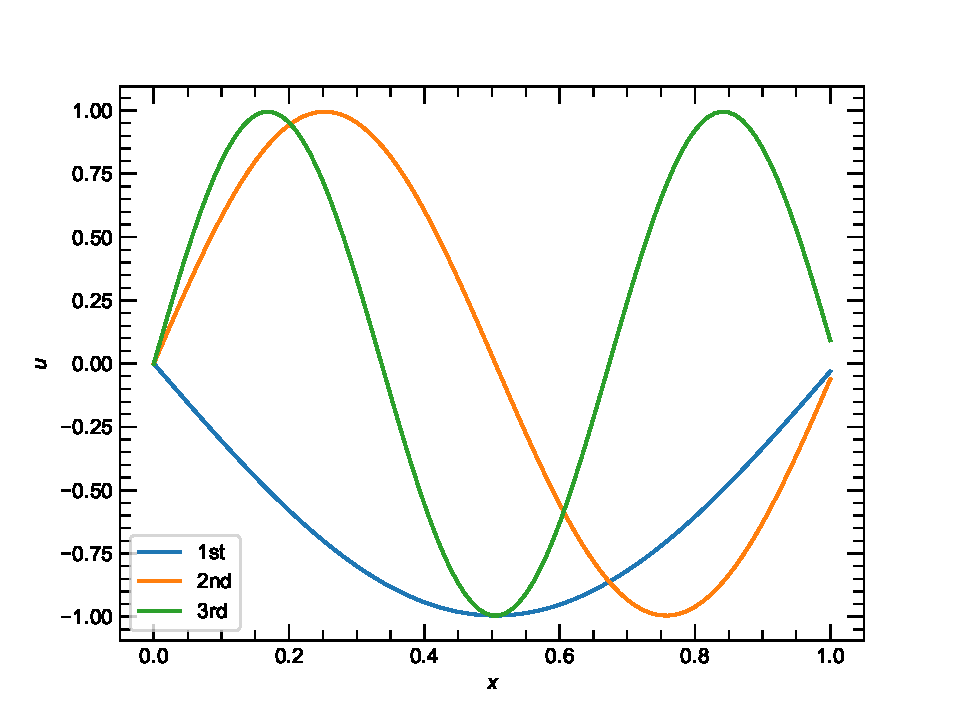
\includegraphics[width=0.8\textwidth]{./figs/eigenfunction.pdf}
    \caption{固有関数}
    \label{fig:eigenfunction}
\end{figure}
\begin{figure}
    \centering
    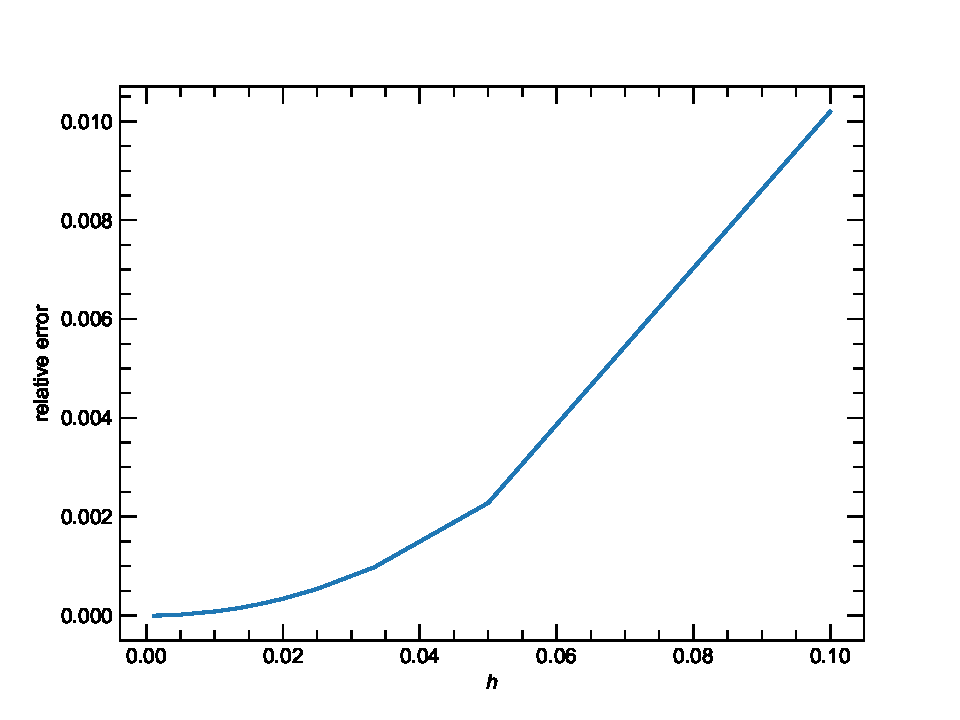
\includegraphics[width=0.8\textwidth]{./figs/convergence.pdf}
    \caption{エネルギー収束の様子。横軸は刻み幅、縦軸はエネルギーの相対誤差。}
    \label{fig:convergence}
\end{figure}
\begin{figure}
    \centering
    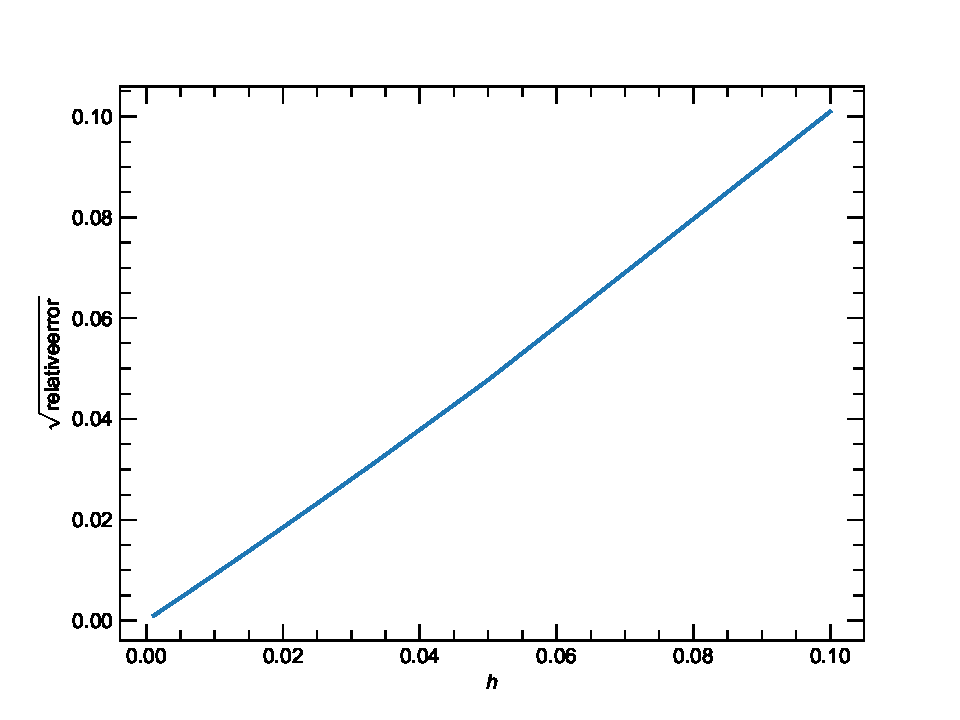
\includegraphics[width=0.8\textwidth]{./figs/convergence_sqrt.pdf}
    \caption{エネルギー収束の様子。横軸は刻み幅、縦軸はエネルギーの相対誤差の平方根。}
    \label{fig:convergence_sqrt}
\end{figure}
\subsubsection{$v\propto1/x$の場合}
固有値方程式は
\begin{align}
    \qty(\dv[2]{x} + \frac{v_0}{x})f &= \lambda f\notag\\
    \qty(x^2\dv[2]{x} + xv_0)f &= \lambda x^2 f
\end{align}
弱形式
にすると、
\begin{align}
    \int_0^L g\qty(x^2\dv[2]{x} + xv_0)f\dd x &= \int_0^L g\lambda x^2 f\dd x\notag\\
    \int_0^L\qty( -\dv{g x^2}{x}\dv{f}{x} + gxv_0f)\dd x &= \int_0^L g\lambda x^2 f\dd x\notag\\
    \int_0^L\qty( - x^2\dv{g}{x}\dv{f}{x} - 2gx\dv{f}{x} + gxv_0f)\dd x &= \int_0^L g\lambda x^2 f\dd x
\end{align}
補完関数
\begin{align}
    N_p(x) = 
    \begin{cases}
        \dfrac{x-x_{p-1}}{h_{p-1}}&x_{p-1}<x<x_p,\\
        \dfrac{x_{p+1} - x}{h_p}&x_{p}<x<x_{p+1},\\
        0&\text{otherwise},
    \end{cases}
\end{align}
を導入する。$g(x) = \sum_{p=1}^N g_pN_p(x)$, $f(x) = \sum_{q=1}^N f_qN_q(x)$と近似すると、
\begin{align}
    -\int_0^L x^2\dv{g}{x}\dv{f}{x}\dd{x}
     =& -\sum_{p, q}\bigg(\delta_{p - 1, q}\dfrac{-1}{h_{p-1}}\cdot\dfrac{1}{h_{p-1}}\cdot h_{p-1}
      + \delta_{q, p}\qty(\dfrac{1}{h_{p-1}}\cdot\dfrac{1}{h_{p-1}}\cdot h_{p-1} + \dfrac{-1}{h_{p}}\cdot\dfrac{-1}{h_{p}}\cdot h_{p})\notag\\
      &+ \delta_{q, p + 1}\dfrac{1}{h_{p}}\cdot\dfrac{-1}{h_{p}}\cdot h_{p}
      \bigg)\notag\\
     =& \sum_{p, q}\bigg(\delta_{q, p - 1}\dfrac{1}{h_{p-1}}
      + \delta_{q, p}\qty(\dfrac{-1}{h_{p-1}} + \dfrac{-1}{h_{p}})+ \delta_{q, p + 1}\dfrac{1}{h_{p}}
      \bigg),
\end{align}
\begin{align}
    \int_0^L gf\dd{x}
     =& \sum_{p, q}\bigg(\delta_{q, p - 1}\int_{x_{p-1}}^{x_p}\dfrac{x_{p} - x}{h_{p-1}}\cdot\dfrac{x-x_{p-1}}{h_{p-1}}\dd{x}\notag\\
      &+ \delta_{q, p}\qty(\int_{x_{p-1}}^{x_p}\dfrac{x-x_{p-1}}{h_{p-1}}\cdot\dfrac{x-x_{p-1}}{h_{p-1}}\dd{x}
       + \int_{x_{p}}^{x_{p+1}}\dfrac{x_{p+1} - x}{h_{p}}\cdot\dfrac{x_{p+1} - x}{h_{p}}\dd{x})\notag\\
      &+ \delta_{q, p + 1}\int_{x_{p}}^{x_{p+1}}\dfrac{x-x_{p}}{h_{p}}\cdot\dfrac{x_{p+1} -x}{h_{p}}\cdot h_{p}
      \bigg)\notag\\
      =& \sum_{p, q}\bigg(\delta_{q, p - 1}\dfrac{h_{p-1}}{6}
      + \delta_{q, p}\qty(\dfrac{h_{p-1}}{3} + \dfrac{h_{p}}{3})+ \delta_{q, p + 1}\dfrac{h_{p}}{6}\bigg)
\end{align}
\end{document}
